\documentclass[preprint,12pt,aps,pra,showkeys,amsmath,amssymb,superscriptaddress,floatfix]{revtex4-2}
\usepackage[T1]{fontenc}
\usepackage[utf8]{inputenc}
\usepackage{amsmath,amssymb,amsthm,mathtools,mathrsfs}
\usepackage{microtype,booktabs,enumitem}
\usepackage{xcolor,tikz,etoolbox}
\usepackage[skins,breakable]{tcolorbox}
\usepackage{needspace}
% Keep diagram geometry independent of REVTeX preprint body spacing.
\AtBeginEnvironment{tikzpicture}{\linespread{1}\selectfont}
\usetikzlibrary{arrows.meta,positioning,calc,fit,decorations.pathreplacing}
\usepackage{graphicx}
\usepackage{hyperref}

\definecolor{MMBlue}{RGB}{0,82,155}
\definecolor{MMOrange}{RGB}{200,80,0}
\tikzset{
 mmnode/.style={draw=MMBlue,rounded corners=2pt,fill=MMBlue!4,align=left,execute at begin node={\raggedright},text width=5cm,font=\fontsize{10}{12}\selectfont,inner sep=6pt},
 mmimport/.style={mmnode,draw=black!65,fill=black!4},
 mmcandidate/.style={mmnode,draw=MMOrange,dashed,fill=MMOrange!5},
 mmrejected/.style={mmnode,draw=black,densely dotted,fill=black!8},
 mmproof/.style={->,thick,MMBlue},
 mmflow/.style={->,semithick,black!70},
 mmrepair/.style={->,dashed,thick,MMOrange},
 mmcandidatearrow/.style={->,dashed,semithick,MMOrange},
 mmnote/.style={font=\scriptsize,fill=white,inner sep=2pt,align=center}}

\usepackage[section]{placeins}
\setlength{\emergencystretch}{3em}
\setlist{itemsep=3pt,topsep=4pt}
\newtheorem{theorem}{Theorem}[section]
\newtheorem{proposition}[theorem]{Proposition}
\newtheorem{lemma}[theorem]{Lemma}
\newtheorem{corollary}[theorem]{Corollary}
\theoremstyle{definition}
\newtheorem{definition}[theorem]{Definition}
\newtheorem{example}[theorem]{Example}
\theoremstyle{remark}
\newtheorem{remark}[theorem]{Remark}
% Avoid isolated statement headings and single-line paragraph fragments.
\BeforeBeginEnvironment{theorem}{\Needspace{6\baselineskip}}
\BeforeBeginEnvironment{definition}{\Needspace{5\baselineskip}}
\BeforeBeginEnvironment{proposition}{\Needspace{5\baselineskip}}
\BeforeBeginEnvironment{lemma}{\Needspace{5\baselineskip}}
\BeforeBeginEnvironment{corollary}{\Needspace{5\baselineskip}}
\clubpenalty=5000
\widowpenalty=5000
\newcommand{\R}{\mathbb R}\newcommand{\Z}{\mathbb Z}\newcommand{\N}{\mathbb N}
\newcommand{\Pa}{\operatorname{Pa}}\newcommand{\Desc}{\operatorname{Desc}}
\newcommand{\cl}{\operatorname{cl}}\newcommand{\cost}{\operatorname{cost}}
\newcommand{\status}{\operatorname{status}}
% Faculty cards: a visual rail groups the five faculties within one agent.
% The rail has no arrowhead and does not represent a proof dependency.
\newcommand{\mmfacultybadge}[1]{%
 \node[circle,draw=MMBlue,line width=1pt,fill=white,
 minimum size=7mm,inner sep=0pt,font=\sffamily\small\bfseries,text=MMBlue]
 at ([xshift=15pt,yshift=-15pt]frame.north west) {#1};}
\newcommand{\mmfacultyrail}{%
 \draw[MMBlue!80,line width=1pt]
 ([xshift=15pt,yshift=2pt]frame.north west)--
 ([xshift=15pt,yshift=-2pt]frame.south west);}
\newtcolorbox{mmfacultybox}[2]{enhanced,breakable,
 colback=MMBlue!4,colframe=MMBlue!4,boxrule=0pt,arc=3pt,
 left=39pt,right=9pt,top=4pt,bottom=4pt,
 before skip=2pt,after skip=2pt,
 fontupper=\small\linespread{1.1}\selectfont,
 overlay unbroken={\mmfacultyrail\mmfacultybadge{#1}},
 overlay first={\mmfacultyrail\mmfacultybadge{#1}},
 overlay middle={\mmfacultyrail},overlay last={\mmfacultyrail}}
\newcommand{\mmfaculty}[3]{%
 \begin{mmfacultybox}{#1}{#2}
 {\sffamily\bfseries\color{MMBlue}#2}\par\smallskip #3
 \end{mmfacultybox}}
\newcommand{\agent}[9]{%
 \Needspace{8\baselineskip}
 \subsubsection{#1}
 \noindent\textbf{Object.} #2\par
 \noindent\textbf{Role.} #3\par\smallskip
 \mmfaculty{E}{Ego}{#4}
 \mmfaculty{M}{Memory}{#5}
 \mmfaculty{I}{Intellect}{#6}
 \mmfaculty{S}{Sense}{#7}
 \mmfaculty{A}{Action}{#8}
 \smallskip\noindent #9\par}

\usepackage{longtable,array,calc}
\providecommand{\tightlist}{\setlength{\itemsep}{2pt}\setlength{\parskip}{0pt}}
\makeatletter
\def\frontmatter@abstract@produce{\par\addvspace{\frontmatter@preabstractspace}%
\begingroup\prep@absbox\unvbox\absbox\post@absbox\endgroup
\addvspace{\frontmatter@postabstractspace}}
\makeatother
\newcommand{\field}[2]{\par\smallskip\noindent\textbf{#1.} #2\par}
\setlength{\emergencystretch}{5em}
\AtBeginEnvironment{verbatim}{\small\linespread{1.0}\selectfont}


\hypersetup{colorlinks=true,linkcolor=MMBlue,urlcolor=MMBlue,pdfauthor={Dibakar Sigdel}}

\begin{document}

\title{d'Alembert's Formula and Finite Propagation\\[4pt]\large An End-to-End Meta-Math Walkthrough}

\author{Dibakar Sigdel}

\affiliation{Mindverse Computing LLC, Lynnwood, WA 98087, USA}

\date{October 2026}

\begin{abstract}

Characteristic coordinates factor the wave operator. The initial
displacement fixes the sum of the two traveling waves; the initial
velocity fixes their derivative difference. The report presents the
target theorem, declared imports, a dependency graph, five-faculty node
contracts, a continuous proof, a worked example, and a hypothesis-repair
audit. It is an authored mathematical exposition, not a deployed-agent
transcript or a formal proof-assistant certificate.

\end{abstract}\maketitle\linespread{1.12}\selectfont

\noindent\textbf{PDE-05 / Partial Differential Equations / Report v1}

\section{Target and import contract}

\begin{theorem}

For \(c>0\), \(f\in C^2(\mathbb R)\) and \(g\in C^1(\mathbb R)\), prove
that the unique \(C^2\) solution on \(\mathbb R\times[0,\infty)\) of
\(u_{tt}=c^2u_{xx}\), \(u(x,0)=f(x)\), \(u_t(x,0)=g(x)\), is
\(u(x,t)=\tfrac12[f(x-ct)+f(x+ct)]+\tfrac1{2c}\int_{x-ct}^{x+ct}g(s)ds\).
Prove that \(u(x,t)\) depends only on the initial data in
\([x-ct,x+ct]\); compactly supported initial data in \([-R,R]\) yield
support inside \([-R-ct,R+ct]\).

\end{theorem}

\subsection{Foundations and permitted imports}

Use the chain rule, the fundamental theorem for variable-endpoint
integrals, and integration of \(U_{\xi\eta}=0\) in characteristic
coordinates. The latter integration is proved below on the half-plane
corresponding to \(t>0\); no assumption that the solution separates
globally is imported. \(C^2\) at \(t=0\) means the derivatives extend
continuously from the half-plane.

\clearpage\section{Node interaction workflow}

\begin{center}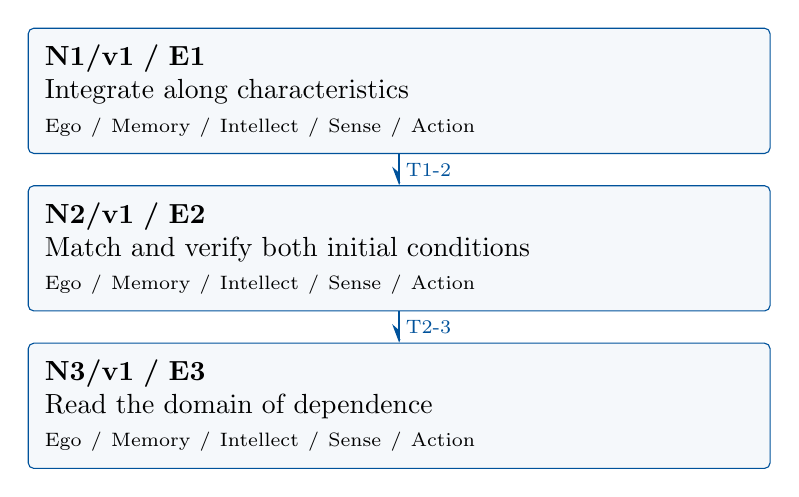
\begin{tikzpicture}[>=Stealth,x=1cm,y=1cm]

\node[mmnode,text width=9cm,minimum height=1.25cm] (N1) at (0,0.0) {\textbf{N1/v1 / E1}\\Integrate along characteristics\\{\scriptsize Ego / Memory / Intellect / Sense / Action}};

\node[mmnode,text width=9cm,minimum height=1.25cm] (N2) at (0,-2.0) {\textbf{N2/v1 / E2}\\Match and verify both initial conditions\\{\scriptsize Ego / Memory / Intellect / Sense / Action}};

\node[mmnode,text width=9cm,minimum height=1.25cm] (N3) at (0,-4.0) {\textbf{N3/v1 / E3}\\Read the domain of dependence\\{\scriptsize Ego / Memory / Intellect / Sense / Action}};

\draw[mmproof] (N1.south) -- node[mmnote,right] {T1-2} (N2.north);

\draw[mmproof] (N2.south) -- node[mmnote,right] {T2-3} (N3.north);

\end{tikzpicture}\end{center}

Each box is one mathematical agent containing all five faculties. Blue
arrows carry the versioned exports listed below. The layout gives a
reading order; only drawn arrows assert dependencies. Diagnostic repair
is separate from the proof DAG.

\subsection{Versioned evidence-transfer ledger}

\begingroup\small\linespread{1.05}\selectfont

\Needspace{5\baselineskip}\field{T1-2: N1/E1/v1 to N2}{Every candidate has the form \(u(x,t)=A(x-ct)+B(x+ct)\) for \(t>0\),
with \(C^2\) functions \(A,B\).}

\field{Receiving activity}{N2.1}

\field{Compatibility}{E1/v1 and \(f,g\) on the initial line. Check: The initial velocity fixes
opposite signs for the two waves; the integral coefficient is
\(1/(2c)\).}

\Needspace{5\baselineskip}\field{T2-3: N2/E2/v1 to N3}{The displayed formula is the only possible solution and is a \(C^2\)
solution with the prescribed data.}

\field{Receiving activity}{N3.1}

\field{Compatibility}{E2/v1 and the explicit endpoints and integral interval. Check: Finite
propagation is a support statement in space-time; it does not assert
that the solution itself stays constant inside the cone.}

\endgroup

\clearpage\section{Agent roles and five-faculty activities}\begingroup\small\linespread{1.05}\selectfont\setlist{itemsep=1pt,topsep=2pt}

\subsection{N1/v1: Integrate along characteristics}

\field{Object and role}{Factor the differential operator and integrate its vanishing mixed
derivative on \(\eta>\xi\). \textbf{Local obligation:} Every candidate
has the form \(u(x,t)=A(x-ct)+B(x+ct)\) for \(t>0\), with \(C^2\)
functions \(A,B\).}

\field{Inputs}{Any \(C^2\) candidate solution, with \(\xi=x-ct\), \(\eta=x+ct\), and
\(U(\xi,\eta)=u((\xi+\eta)/2,(\eta-\xi)/(2c))\).}

\mmfaculty{E}{Ego}{Publish E1/v1 only after establishing this obligation: Every candidate
has the form \(u(x,t)=A(x-ct)+B(x+ct)\) for \(t>0\), with \(C^2\)
functions \(A,B\).}

\mmfaculty{M}{Memory}{Any \(C^2\) candidate solution, with \(\xi=x-ct\), \(\eta=x+ct\), and
\(U(\xi,\eta)=u((\xi+\eta)/2,(\eta-\xi)/(2c))\). Retain the stated
assumptions and import versions.}

\mmfaculty{I}{Intellect}{Factor the differential operator and integrate its vanishing mixed
derivative on \(\eta>\xi\).}

\mmfaculty{S}{Sense}{The transformed domain is a half-plane; justify separation there rather
than presuming a rectangular global domain.}

\mmfaculty{A}{Action}{Carry out activities N1.1--N1.2 below, retaining each calculation and
construction as evidence.}

\smallskip\noindent\textbf{Numbered mathematical activities}

\begin{enumerate}[label=N1.\arabic*,leftmargin=3.4em]

\item The chain rule gives \(u_{tt}-c^2u_{xx}=-4c^2U_{\xi\eta}\), so the mixed
derivative vanishes on \(\eta>\xi\). For fixed \(\xi\),
\(U_\xi(\xi,\eta)\) is constant on the connected interval \(\eta>\xi\).
Denote it by \(a(\xi)\); locally one can evaluate at a fixed admissible
\(\eta\), so \(a\) is \(C^1\).

\item Choose an antiderivative \(A\) of \(a\). Then \(U-A\) has zero \(\xi\)
derivative. For each fixed \(\eta\), the interval \(\xi<\eta\) is
connected, so \(U(\xi,\eta)-A(\xi)\) depends only on \(\eta\); call it
\(B(\eta)\). Local evaluation shows \(B\) is \(C^2\). Thus \(U=A+B\) on
the half-plane. Continuity extends the corresponding identities to
\(t=0\).

\end{enumerate}

\field{Export E1/v1}{Every candidate has the form \(u(x,t)=A(x-ct)+B(x+ct)\) for \(t>0\),
with \(C^2\) functions \(A,B\).}

\field{Acceptance gate}{The transformed domain is a half-plane; justify separation there rather
than presuming a rectangular global domain.}

\field{Targeted repair}{If separation is asserted without checking the transformed domain, use
connected characteristic intervals to integrate each derivative.
Withhold this export and recheck its descendants after a versioned
correction.}

\clearpage

\subsection{N2/v1: Match and verify both initial conditions}

\field{Object and role}{Solve for the derivatives of the traveling-wave components and
substitute their antiderivatives. \textbf{Local obligation:} The
displayed formula is the only possible solution and is a \(C^2\)
solution with the prescribed data.}

\field{Inputs}{E1/v1 and \(f,g\) on the initial line. Incoming proof exports: E1/v1 at
N2.1.}

\mmfaculty{E}{Ego}{Publish E2/v1 only after establishing this obligation: The displayed
formula is the only possible solution and is a \(C^2\) solution with the
prescribed data.}

\mmfaculty{M}{Memory}{E1/v1 and \(f,g\) on the initial line. Incoming proof exports: E1/v1 at
N2.1. Retain the stated assumptions and import versions.}

\mmfaculty{I}{Intellect}{Solve for the derivatives of the traveling-wave components and
substitute their antiderivatives.}

\mmfaculty{S}{Sense}{The initial velocity fixes opposite signs for the two waves; the
integral coefficient is \(1/(2c)\).}

\mmfaculty{A}{Action}{Carry out activities N2.1--N2.2 below, retaining each calculation and
construction as evidence.}

\smallskip\noindent\textbf{Numbered mathematical activities}

\begin{enumerate}[label=N2.\arabic*,leftmargin=3.4em]

\item At \(t=0\), \(A(x)+B(x)=f(x)\) and \(-cA'(x)+cB'(x)=g(x)\).
Differentiating the first identity and solving gives \(A'=(f'-g/c)/2\),
\(B'=(f'+g/c)/2\). If \(G(x)=\int_0^x g(s)ds\), integration gives
\(A=f/2-G/(2c)+C\) and \(B=f/2+G/(2c)-C\).

\item Substitution at \(x-ct\) and \(x+ct\) cancels \(C\) and gives
d'Alembert's formula. Conversely these \(A,B\) are \(C^2\) because
\(f\in C^2\) and \(G\in C^2\). Each traveling wave satisfies
\(u_{tt}=c^2u_{xx}\) by direct differentiation, and the two initial
identities hold. Thus a solution exists and every candidate equals it,
proving uniqueness.

\end{enumerate}

\field{Export E2/v1}{The displayed formula is the only possible solution and is a \(C^2\)
solution with the prescribed data.}

\field{Acceptance gate}{The initial velocity fixes opposite signs for the two waves; the
integral coefficient is \(1/(2c)\).}

\field{Targeted repair}{If only the initial displacement is matched, compute the time derivative
at zero and fix the relative sign and factor using \(g\). Withhold this
export and recheck its descendants after a versioned correction.}

\clearpage

\subsection{N3/v1: Read the domain of dependence}

\field{Object and role}{Locate every initial value used by the solution and compare two data
sets on that interval. \textbf{Local obligation:} Only initial data in
\([x-ct,x+ct]\) affect \(u(x,t)\), and the stated support bound holds.}

\field{Inputs}{E2/v1 and the explicit endpoints and integral interval. Incoming proof
exports: E2/v1 at N3.1.}

\mmfaculty{E}{Ego}{Publish E3/v1 only after establishing this obligation: Only initial data
in \([x-ct,x+ct]\) affect \(u(x,t)\), and the stated support bound
holds.}

\mmfaculty{M}{Memory}{E2/v1 and the explicit endpoints and integral interval. Incoming proof
exports: E2/v1 at N3.1. Retain the stated assumptions and import
versions.}

\mmfaculty{I}{Intellect}{Locate every initial value used by the solution and compare two data
sets on that interval.}

\mmfaculty{S}{Sense}{Finite propagation is a support statement in space-time; it does not
assert that the solution itself stays constant inside the cone.}

\mmfaculty{A}{Action}{Carry out activities N3.1--N3.2 below, retaining each calculation and
construction as evidence.}

\smallskip\noindent\textbf{Numbered mathematical activities}

\begin{enumerate}[label=N3.\arabic*,leftmargin=3.4em]

\item The formula uses \(f\) only at the two endpoints and \(g\) only inside
the closed interval. Therefore two admissible initial data sets agreeing
on that interval produce the same value at \((x,t)\).

\item If \(f,g\) vanish outside \([-R,R]\) and \(x>R+ct\), then the entire
integration interval and both endpoints lie to the right of \(R\), so
every term is zero. The same holds for \(x<-R-ct\). Hence the support at
time \(t\) is contained in the enlarged interval, proving finite
propagation.

\end{enumerate}

\field{Export E3/v1}{Only initial data in \([x-ct,x+ct]\) affect \(u(x,t)\), and the stated
support bound holds.}

\field{Acceptance gate}{Finite propagation is a support statement in space-time; it does not
assert that the solution itself stays constant inside the cone.}

\field{Targeted repair}{If the support is claimed to stay inside its initial interval, expand
the interval by the characteristic distance \(ct\). Withhold this export
and recheck its descendants after a versioned correction.}

\endgroup\clearpage\section{Continuous mathematical proof}\label{sec:proof}

\subsection{N1 --- Integrate along
characteristics}\label{n1-integrate-along-characteristics}

\begin{enumerate}
\def\labelenumi{\arabic{enumi}.}
\item
  \textbf{N1.1.} The chain rule gives
  \(u_{tt}-c^2u_{xx}=-4c^2U_{\xi\eta}\), so the mixed derivative
  vanishes on \(\eta>\xi\). For fixed \(\xi\), \(U_\xi(\xi,\eta)\) is
  constant on the connected interval \(\eta>\xi\). Denote it by
  \(a(\xi)\); locally one can evaluate at a fixed admissible \(\eta\),
  so \(a\) is \(C^1\).
\item
  \textbf{N1.2.} Choose an antiderivative \(A\) of \(a\). Then \(U-A\)
  has zero \(\xi\) derivative. For each fixed \(\eta\), the interval
  \(\xi<\eta\) is connected, so \(U(\xi,\eta)-A(\xi)\) depends only on
  \(\eta\); call it \(B(\eta)\). Local evaluation shows \(B\) is
  \(C^2\). Thus \(U=A+B\) on the half-plane. Continuity extends the
  corresponding identities to \(t=0\).
\end{enumerate}

\subsection{N2 --- Match and verify both initial
conditions}\label{n2-match-and-verify-both-initial-conditions}

\begin{enumerate}
\def\labelenumi{\arabic{enumi}.}
\item
  \textbf{N2.1.} At \(t=0\), \(A(x)+B(x)=f(x)\) and
  \(-cA'(x)+cB'(x)=g(x)\). Differentiating the first identity and
  solving gives \(A'=(f'-g/c)/2\), \(B'=(f'+g/c)/2\). If
  \(G(x)=\int_0^x g(s)ds\), integration gives \(A=f/2-G/(2c)+C\) and
  \(B=f/2+G/(2c)-C\).
\item
  \textbf{N2.2.} Substitution at \(x-ct\) and \(x+ct\) cancels \(C\) and
  gives d'Alembert's formula. Conversely these \(A,B\) are \(C^2\)
  because \(f\in C^2\) and \(G\in C^2\). Each traveling wave satisfies
  \(u_{tt}=c^2u_{xx}\) by direct differentiation, and the two initial
  identities hold. Thus a solution exists and every candidate equals it,
  proving uniqueness.
\end{enumerate}

\subsection{N3 --- Read the domain of
dependence}\label{n3-read-the-domain-of-dependence}

\begin{enumerate}
\def\labelenumi{\arabic{enumi}.}
\item
  \textbf{N3.1.} The formula uses \(f\) only at the two endpoints and
  \(g\) only inside the closed interval. Therefore two admissible
  initial data sets agreeing on that interval produce the same value at
  \((x,t)\).
\item
  \textbf{N3.2.} If \(f,g\) vanish outside \([-R,R]\) and \(x>R+ct\),
  then the entire integration interval and both endpoints lie to the
  right of \(R\), so every term is zero. The same holds for \(x<-R-ct\).
  Hence the support at time \(t\) is contained in the enlarged interval,
  proving finite propagation.
\end{enumerate}

\hfill$\square$

\section{Worked orchestration}

For \(c=1\), \(f=0\), and \(g(s)=\cos s\), the formula gives
\(u(x,t)=(\sin(x+t)-\sin(x-t))/2=\cos x\sin t\). Then
\(u_{tt}=-\cos x\sin t=u_{xx}\), \(u(x,0)=0\), and \(u_t(x,0)=\cos x\).

\subsection{Boundary and hypothesis audit}

Initial displacement alone does not determine a wave solution. Both
\(u=0\) and \(u=t\) have zero initial displacement and satisfy the wave
equation, but their initial velocities differ. Prescribing both \(f\)
and \(g\) is essential.

\section{Illustrative failure and repair}

The following is an authored diagnostic scenario. Changed assumptions
define a new contract; they do not retroactively prove the original
statement.

\subsection{Rejected argument, diagnosis, and correction}
\textbf{Rejected N2 solution:} keep only \([f(x-ct)+f(x+ct)]/2\) even
when \(g\ne0\). Its time derivative at zero is zero, so it fails the
velocity datum. \textbf{Diagnosis:} Action matched only half the initial
contract. \textbf{Repair:} solve the two derivative equations and add
the integral of \(g\) with coefficient \(1/(2c)\). Recheck the PDE, both
initial data, and the interval used for finite propagation.

\subsection{Publication and reuse}
The corrected export retains its explicit assumptions. A hypothetical
revision receives a new version, and each consuming activity is
rechecked; this scenario is not a recorded runtime event. \textbf{Next
direction:} Extend characteristic reasoning to inhomogeneous forcing
with Duhamel's principle, using a new source-term contract.

\par\medskip\begingroup\small\linespread{1.0}\selectfont\noindent\textbf{Provenance.} This authored proof is complete relative to its declared imports. Reuse
each export with its assumptions, proof, and version. The original
Markdown remains available for comparison.
\par\endgroup

\par\smallskip\begingroup\small\linespread{1.0}\selectfont\noindent\textbf{Further reading.} \href{https://math.stanford.edu/~lms/lecs-on-pde.pdf}{Leon Simon,
Lectures on PDE}, for elliptic, weak, and parabolic methods. Classical
calculus and the explicitly stated Hilbert-space imports are used below;
the displayed PDE arguments are developed in full.\par\endgroup

\end{document}
